\chapter{爆发、瞬变和多信使量子天文学}
\label{chap:13}

\begin{chapteropening}
瞬变源把天体物理过程压缩到一个可观测的时间轴上。新星和超新星给出膨胀速度、距离和角尺度的联立问题；GRB 余辉追踪相对论激波、同步辐射和喷流角；千新星同时牵涉引力波定位、伽马射线延迟、颜色演化和 \(r\)-process ejecta；TDE 则从黑洞质量、回落率和再处理光球进入观测。平均光变曲线不够用；带有时间、频率、偏振、空间通道和触发来源的事件表才能同时约束触发时刻、背景、膨胀几何、颜色演化和多信使延迟 \citep{2014Natur.514..339C,2014Sci...345..554A,2008Sci...321..223S,1998ApJ...497L..17S,2004RvMP...76.1143P,2017PhRvL.119p1101A,2017ApJ...848L..12A,2017Natur.551...75S,2021ARA&A..59...21G}。
\end{chapteropening}

\section{为什么瞬变从触发似然开始}

一次瞬变观测从触发开始，但触发本身已经是一个统计推断。对第 \(k\) 个探测通道，事件率可以写成
\begin{equation}
  \lambda_k(t)=b_k(t)+A_{{\rm eff},k}(t)
  \int R_k(\nu,p,t)\,F_\nu(t,p)\,d\nu ,
  \label{eq:ch13-rate-response}
\end{equation}
\begin{formulaexplain}
\(\lambda_k(t)\) 是第 \(k\) 个通道的事件率，\(b_k\) 是背景，\(A_{\rm eff}\) 和 \(R_k\) 描述仪器响应，\(F_\nu\) 是源通量。触发从模型事件率开始。
\end{formulaexplain}
其中 \(\lambda_k\) 的单位是 \(\mathrm{s^{-1}}\)，\(b_k\) 是天光、宿主星系、暗计数和误触发贡献的背景率，\(A_{{\rm eff},k}\) 是有效面积，\(R_k\) 是包含带宽、量子效率、偏振选择和时间响应的仪器响应，\(F_\nu(t,p)\) 是源在频率 \(\nu\) 和偏振态 \(p\) 上的光子通量。光学瞬变的单通道事件率可以从低于 \(1\,\mathrm{s^{-1}}\) 到 \(10^6\,\mathrm{s^{-1}}\)；高能探测器常以较粗能道记录事件，射电和光学快探测器则更强调亚微秒到纳秒时间戳。

如果只关心一个快升慢降的触发窗口，常用的第一模型是
\begin{equation}
  \lambda(t)=b+A\exp\!\left[-\frac{t-t_0}{\tau}\right]H(t-t_0),
  \label{eq:ch13-exponential-rate}
\end{equation}
\begin{formulaexplain}
\(\lambda(t)\) 是快升慢降的事件率模型，\(b\) 是背景，\(A\) 是初始超额率，\(t_0\) 是起始时刻，\(\tau\) 是衰减时间。\(H\) 保证触发前没有该源项。
\end{formulaexplain}
\(b\) 是背景率，\(A\) 是触发后源的初始超额率，\(t_0\) 是物理起始时刻，\(\tau\) 是衰减时标，\(H\) 是阶跃函数。这里的 \(t\) 可用秒、小时或天，只要 \(A\) 和 \(b\) 用同一时间单位的倒数。GRB prompt emission 的 \(\tau\) 可以是 \(10^{-2}-10^2\,\mathrm{s}\)，光学 afterglow 的有效衰减时间通常是小时到天，新星和 TDE 的 \(\tau\) 可以到数十天或数百天。

事件表 \(\{t_j\}\) 对非齐次 Poisson 过程的对数似然为
\begin{equation}
  \ln L=\sum_{j=1}^{N}\ln \lambda(t_j)-\int_{t_{\rm min}}^{t_{\rm max}}\lambda(t)\,dt .
  \label{eq:ch13-poisson-likelihood}
\end{equation}
\begin{formulaexplain}
\(\ln L\) 是非齐次 Poisson 事件表似然。第一项奖励模型在真实光子时刻给出高事件率，第二项惩罚模型在整个窗口里预言过多计数。
\end{formulaexplain}
第一项在真实光子到达时刻评价模型事件率，第二项扣除模型在整个观测窗口内预言的总计数。式中的 \(\ln L\) 可由未分箱事件直接计算；如果把数据先分成很宽的时间 bin，\(t_0\) 和快速上升段的信息会被平均掉。这个形式也适用于带能量、频率和偏振标签的事件，只需把 \(\lambda(t)\) 换成 \(\lambda(t,\nu,p)\)，并把积分扩展到对应坐标。

\begin{figure}[tbp]
\centering
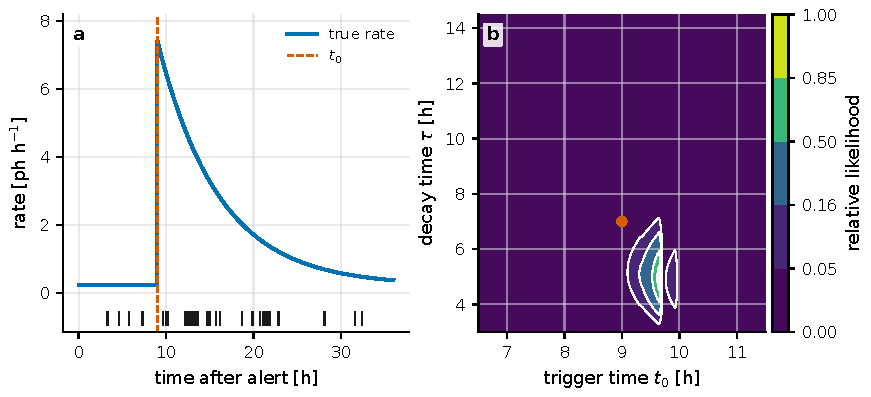
\includegraphics[width=0.92\linewidth]{figures/generated/chapter_13/ch13_transient_event_likelihood.pdf}
\caption{非齐次 Poisson 事件表怎样约束触发时间和衰减时间。左图中的竖线是单个光子到达时刻，蓝线是事件率模型；右图把同一事件表写成 \(t_0\) 和 \(\tau\) 的相对似然面。少量早期光子会强烈限制 \(t_0\)，而晚期背景决定 \(\tau\) 是否被高估。}
\label{fig:chapter-13-event-likelihood}
\end{figure}

触发器通常比较瞬变模型 \(M_{\rm tr}\) 和背景模型 \(M_{\rm bg}\)。用 odds ratio 写成
\begin{equation}
  {\cal O}_{\rm tr,bg}
  =
  \frac{P(M_{\rm tr})}{P(M_{\rm bg})}
  \frac{L(D|M_{\rm tr})}{L(D|M_{\rm bg})},
  \label{eq:ch13-trigger-odds}
\end{equation}
\begin{formulaexplain}
\({\cal O}_{\rm tr,bg}\) 是瞬变模型相对背景模型的 odds ratio。它把先验发生率和数据似然同时放进触发判断。
\end{formulaexplain}
\(D\) 是事件表或图像差分数据，\(P(M)\) 是先验发生率。若背景在窗口 \(\Delta t\) 内的期望计数为 \(\mu_b=b\Delta t\)，单窗口 Poisson false alarm probability 为
\begin{equation}
  P_{\rm FA}(N\ge n)=
  \sum_{m=n}^{\infty}\frac{\mu_b^m e^{-\mu_b}}{m!}.
  \label{eq:ch13-false-alarm}
\end{equation}
\begin{formulaexplain}
\(P_{\rm FA}\) 是背景单独产生 \(n\) 个或更多计数的误触发概率，\(\mu_b\) 是背景期望计数。触发阈值本质上是在控制这个尾概率。
\end{formulaexplain}
实际巡天还要乘以试验次数：时间窗口数、天空像素数、能道数和模板数都会增加误触发。FRB 搜索、伽马射线触发和光学差分巡天都面对同一问题，只是 \(\Delta t\) 从毫秒到天不等，背景从仪器噪声到变量源污染不等 \citep{2013Sci...341...53T,2017ApJ...835...29Y,2020Natur.587...59B,2020Natur.587...54C,2020Natur.581..391M}。

\section{膨胀源怎样把速度、时间和角尺度连起来}

新星和超新星的共同物理图像是一个速度分层的 ejecta。早期光球由光学厚的外层决定；随后谱线形成区向内退，低光学深度的壳层逐渐显露。若膨胀近似 homologous，即半径和速度满足 \(r=v(t-t_0)\)，角半径为
\begin{equation}
  \theta(t)=\frac{v_{\rm exp}(t-t_0)}{D}
  =
  5.8\,{\rm mas}
  \left(\frac{v_{\rm exp}}{10^8\,{\rm cm\,s^{-1}}}\right)
  \left(\frac{t-t_0}{10\,{\rm d}}\right)
  \left(\frac{D}{1\,{\rm kpc}}\right)^{-1}.
  \label{eq:ch13-angular-expansion}
\end{equation}
\begin{formulaexplain}
\(\theta(t)\) 是膨胀源角半径，\(v_{\rm exp}\) 是膨胀速度，\(D\) 是距离。它把谱线速度、爆发时间和角尺度连成几何距离问题。
\end{formulaexplain}
\(\theta\) 可由成像、干涉或模型可见度估计；\(v_{\rm exp}\) 常由谱线的 Doppler 宽度或吸收最低点估计；\(D\) 是距离。新星在 \(D\sim1-5\,\mathrm{kpc}\)、\(v_{\rm exp}\sim10^8\,\mathrm{cm\,s^{-1}}\) 时，几天到几十天内可达到毫角秒尺度。Type Ia 超新星在 \(D\sim10-100\,\mathrm{Mpc}\)、\(v_{\rm exp}\sim10^9\,\mathrm{cm\,s^{-1}}\) 时，十天角半径只有数微角秒。GW170817 类千新星速度可达 \(0.1-0.3c\)，但距离约 \(40\,\mathrm{Mpc}\)，早期角尺度仍在微角秒以下。

\begin{figure}[tbp]
\centering
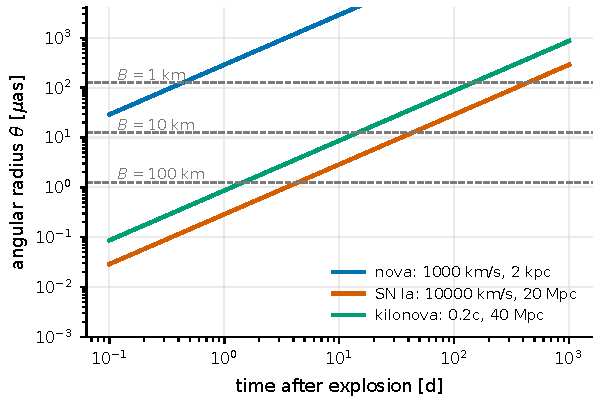
\includegraphics[width=0.92\linewidth]{figures/generated/chapter_13/ch13_expanding_fireball_resolution.pdf}
\caption{膨胀源的角半径由速度、时间和距离共同决定。银河系新星虽然速度低，但距离近，角尺度最快进入毫角秒范围；低红移 Type Ia 超新星和千新星速度更高，却因距离远落在微角秒范围。水平虚线给出 \(\lambda=0.5\,\mu{\rm m}\) 时不同光学基线的 \(\lambda/B\) 标度。}
\label{fig:chapter-13-expansion}
\end{figure}

谱线把速度投影到波长上：
\begin{equation}
  v_{\rm los}\simeq c\,\frac{\lambda_{\rm obs}-\lambda_0}{\lambda_0},
  \label{eq:ch13-doppler-line}
\end{equation}
\begin{formulaexplain}
\(v_{\rm los}\) 是视向速度，\(\lambda_{\rm obs}\) 和 \(\lambda_0\) 是观测与实验室波长。谱线位移把 ejecta 的速度层投影到波长轴上。
\end{formulaexplain}
\(\lambda_0\) 是实验室波长，\(\lambda_{\rm obs}\) 是观测波长。P-Cygni absorption 的蓝端常近似代表外层最快物质，吸收最低点更接近光学深度最大的速度层；发射线半宽则混合了几何、光学深度和密度分布。若每个谱线通道都能测角尺度或相关函数，数据会变成一组 \(\theta(v_{\rm los})\)，可以区分球壳、双锥、赤道环和 polar wind。

强度干涉中，一个圆对称均匀光盘的二阶相关给出 \(|V|^2\)。对应的一阶可见度模长为
\begin{equation}
  |V(B)|=
  \left|
  \frac{2J_1(\pi B\Theta/\lambda)}{\pi B\Theta/\lambda}
  \right|,
  \label{eq:ch13-uniform-disk-visibility}
\end{equation}
\begin{formulaexplain}
\(|V(B)|\) 是均匀圆盘可见度模长，\(\Theta\) 是角直径，\(B\) 是基线，\(\lambda\) 是波长。强度干涉测 \(|V|^2\)，可反推瞬变源角尺度。
\end{formulaexplain}
\(\Theta=2\theta\) 是角直径，\(B\) 是投影基线，\(\lambda\) 是观测波长。这个公式假设圆对称、单波长和无强 limb darkening；真实新星和超新星更常需要薄壳、环、椭球或多组分模型。把角膨胀和谱线速度合并，可以得到 expansion parallax：
\begin{equation}
  D=\frac{v_{\rm exp}(t-t_0)}{\theta(t)}.
  \label{eq:ch13-expansion-parallax}
\end{equation}
\begin{formulaexplain}
\(D\) 是膨胀视差距离。只有当 \(v_{\rm exp}\) 和 \(\theta(t)\) 对应同一物质层时，这个几何距离才不会被速度分层系统偏置。
\end{formulaexplain}
左边的 \(D\) 是几何距离，右边的 \(v_{\rm exp}\) 应和 \(\theta\) 对应同一层物质。若谱线测到的是外层高速吸收，而角尺度来自连续谱光球，距离会系统偏差。

经典新星是白矮星表面的热核爆发，典型 ejecta mass 为 \(10^{-5}-10^{-4}M_\odot\)，速度超过 \(10^3\,\mathrm{km\,s^{-1}}\)。Fermi 发现新星是 GeV \(\gamma\)-ray 源之后，物理图像转向双流结构：慢而密的 equatorial ejecta 被双星轨道塑形，快的 polar wind 撞上它，在内部激波中加速粒子。V959 Mon 的 \(\gamma\)-ray 发射持续约 \(12\,\mathrm{d}\)，高分辨射电成像显示 shock 位于 polar flow 和 equatorial material 的交界，热 ejecta mass 约 \(4\times10^{-5}M_\odot\) \citep{2014Natur.514..339C,2014Sci...345..554A}。在这种源里，\(v_{\rm exp}\) 包含 equatorial 和 polar 两个速度组分；谱线、射电图像和光子事件表要共同拟合。

Type Ia 超新星通常先由亮度校正进入距离问题。Phillips relation 用 \(B\) band 衰减率 \(\Delta m_{15}(B)\) 校正峰值绝对星等；宇宙学应用再把校正后的距离模数写成
\begin{equation}
  \mu = m_B - M_B + \alpha x_1-\beta C+\Delta_{\rm host},
  \label{eq:ch13-snia-distance-modulus}
\end{equation}
\begin{formulaexplain}
\(\mu\) 是距离模数，\(m_B\) 和 \(M_B\) 是观测与标准化峰值星等，\(x_1\) 是光变宽度，\(C\) 是颜色。Type Ia 标准化本质上是在修正光度。
\end{formulaexplain}
\(m_B\) 是观测峰值星等，\(M_B\) 是标准化绝对星等，\(x_1\) 或类似参数描述光变曲线宽度，\(C\) 是颜色，\(\alpha\)、\(\beta\) 和 \(\Delta_{\rm host}\) 由样本拟合。近邻样本中 \(m_B\sim10-16\) 的 Type Ia 可以在小望远镜上得到高信噪光变曲线；宇宙学样本常在 \(m_B\sim22-25\)。如果同时测到角膨胀，就可以用几何距离交叉检查光度距离。这个目标很难，因为十几天的 Type Ia 角直径只有微角秒量级；在长基线光学强度干涉中，它属于难度很高但科学收益明确的瞬变应用 \citep{1993ApJ...413L.105P,1998AJ....116.1009R,1999ApJ...517..565P}。

Type Ia 的偏振告诉我们 ejecta 是否真的近似球对称。Stokes 参数常写为
\begin{equation}
  q=\frac{Q}{I},\qquad
  u=\frac{U}{I},\qquad
  P=\sqrt{q^2+u^2},
  \label{eq:ch13-stokes-polarization}
\end{equation}
\begin{formulaexplain}
\(q,u\) 是归一化 Stokes 参数，\(P\) 是线偏振度。偏振把 ejecta 非球对称和散射几何写进可观测量。
\end{formulaexplain}
\(q\)、\(u\) 和 \(P\) 是无量纲，通常用百分数报告。SN 1999by 在最大光附近有 \(P\simeq0.3-0.8\%\)，Si II \(6150\,\text{\AA}\) 附近有约 \(0.4\%\) 的偏振变化，模型指向约 \(20\%\) 的整体非球对称，并且 Si 层和连续谱大体共享同一对称轴 \citep{2001ApJ...556..302H}。\(\Theta(t)\)、\(v_{\rm exp}\) 和 \(P(t,\lambda)\) 应放在同一个几何模型里解释：角尺度来自光球形状，谱线来自速度层，偏振来自散射几何。

核心坍缩超新星的最早窗口是 shock breakout。激波离表面还有一段距离时，辐射先扩散出来形成 radiative precursor。令 \(d\) 为激波到表面的深度，\(\rho\) 为局部密度，\(\kappa\) 为 opacity，光学深度 \(\tau\simeq\kappa\rho d\)。breakout 条件近似为
\begin{equation}
  t_{\rm diff}\simeq \frac{\tau d}{c}\simeq \frac{d}{v_s},
  \qquad
  \tau\simeq \frac{c}{v_s},
  \label{eq:ch13-shock-breakout-condition}
\end{equation}
\begin{formulaexplain}
\(t_{\rm diff}\) 是辐射扩散时间，\(d\) 是激波到表面的深度，\(v_s\) 是激波速度。breakout 发生在扩散时间赶上动力学时间时。
\end{formulaexplain}
\(v_s\) 是 shock velocity。对红超巨星，\(v_s\sim1-2\times10^9\,\mathrm{cm\,s^{-1}}\)，早期能量主要出现在 extreme UV 或 soft X-ray，光学发现常滞后数天。SNLS-04D2dc 的 GALEX UV 数据显示了 shock 到达表面前的 radiative precursor，并给出 envelope 结构和 progenitor radius 的约束 \citep{2008Sci...321..223S,2011ApJ...727..104C}。这些小时级早期信号要求触发系统压缩 alert、slew、acquisition 和第一轮曝光之间的延迟。

\section{千新星怎样把多信使延迟变成物理约束}

GW170817 给出了多信使瞬变的清楚时间轴。引力波给出 binary neutron star inspiral 的 coalescence time 和距离，Fermi/GBM 与 INTEGRAL 在约 \(1.74\pm0.05\,\mathrm{s}\) 后看到 GRB 170817A，光学 counterpart 在十几小时内被定位，随后 UV/optical/NIR 颜色从蓝快速转红 \citep{2017PhRvL.119p1101A,2017ApJ...848L..13A,2017ApJ...848L..12A,2017ApJ...848L..17C,2017Natur.551...75S,2017ApJ...848L..27T,2017ApJ...848L..24V,2017ApJ...848L..18N,2017Sci...358.1565E,2017ApJ...851L..21V}。

多信使延迟定义为
\begin{equation}
  \Delta t_{a-b}=t_a-t_b .
  \label{eq:ch13-mm-delay}
\end{equation}
\begin{formulaexplain}
\(\Delta t_{a-b}\) 是两个信使或波段的到达时间差。只有把所有时间戳放到同一时标系统中，多信使延迟才有物理意义。
\end{formulaexplain}
\(t_a\) 和 \(t_b\) 是同一时标系统中的到达时间。解释 \(\Delta t\) 时要分成三部分：
\begin{equation}
  \Delta t_{\rm obs}
  =
  \Delta t_{\rm engine}
  +
  \Delta t_{\rm prop}
  +
  \Delta t_{\rm clock}.
  \label{eq:ch13-delay-budget}
\end{equation}
\begin{formulaexplain}
\(\Delta t_{\rm obs}\) 是观测延迟，分成源内发射延迟、传播延迟和时钟/处理误差。这个分解避免把源物理误认为基本传播效应。
\end{formulaexplain}
\(\Delta t_{\rm engine}\) 是源内发射延迟，例如 merger 到 jet breakout 的时间；\(\Delta t_{\rm prop}\) 是传播延迟，可用于约束传播速度差或等效质量；\(\Delta t_{\rm clock}\) 是仪器时钟和数据处理误差。若源距 \(D\) 已知，传播速度差的数量级为
\begin{equation}
  \frac{|\Delta v|}{c}
  \lesssim
  \frac{|\Delta t_{\rm prop}|}{D/c}
  =
  2.4\times10^{-16}
  \left(\frac{\Delta t_{\rm prop}}{1\,{\rm s}}\right)
  \left(\frac{D}{40\,{\rm Mpc}}\right)^{-1}.
  \label{eq:ch13-speed-difference}
\end{equation}
\begin{formulaexplain}
\(|\Delta v|/c\) 是传播速度差的相对量级，\(D/c\) 是光行时。远距离让秒级传播延迟对应极小的速度差约束。
\end{formulaexplain}
这个公式左边不能直接把 \(1.74\,\mathrm{s}\) 全部当作传播延迟，因为 GRB 发射本身可能晚于 merger。它的用处是把“可容许的新传播效应”放到正确数量级上。

\begin{figure}[tbp]
\centering
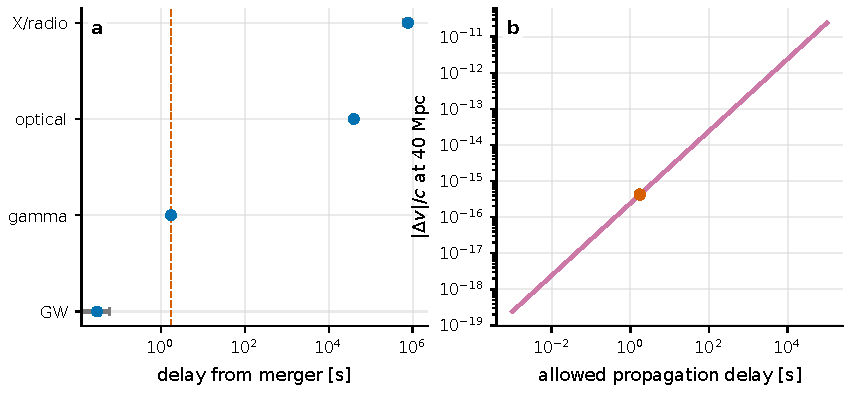
\includegraphics[width=0.92\linewidth]{figures/generated/chapter_13/ch13_multimessenger_delay.pdf}
\caption{多信使延迟的两个读法。左图比较 merger 后不同通道的到达时间：GW 和 \(\gamma\)-ray 位于秒尺度，光学 counterpart 通常受定位和昼夜周期限制，X-ray/radio 可在天到月尺度出现。右图把传播延迟换算成 \(40\,\mathrm{Mpc}\) 距离上的 \(|\Delta v|/c\) 数量级；源内发射延迟越不确定，传播约束越保守。}
\label{fig:chapter-13-mm-delay}
\end{figure}

千新星的光度来自 neutron-rich ejecta 中 \(r\)-process 放射性衰变热化。一个常用标度是
\begin{equation}
  \dot q(t)\simeq
  2\times10^{10}
  \left(\frac{t}{1\,{\rm d}}\right)^{-1.3}
  {\rm erg\,s^{-1}\,g^{-1}},
  \label{eq:ch13-rprocess-heating}
\end{equation}
\begin{formulaexplain}
\(\dot q(t)\) 是 \(r\)-process 物质单位质量加热率。千新星光度的能量源来自这项放射性衰变热化。
\end{formulaexplain}
\(\dot q\) 是单位质量加热率。进入光度的是 \(\epsilon_{\rm th}M_{\rm ej}\dot q\)，其中 \(\epsilon_{\rm th}<1\) 是热化效率，\(M_{\rm ej}\) 是 ejecta mass。扩散时间决定光变峰值：
\begin{equation}
  t_{\rm pk}\simeq
  \left(\frac{\kappa M_{\rm ej}}{4\pi v_{\rm ej}c}\right)^{1/2}
  =
  0.6\,{\rm d}
  \left(\frac{\kappa}{0.5\,{\rm cm^2\,g^{-1}}}\right)^{1/2}
  \left(\frac{M_{\rm ej}}{0.01M_\odot}\right)^{1/2}
  \left(\frac{v_{\rm ej}}{0.3c}\right)^{-1/2}.
  \label{eq:ch13-kilonova-diffusion}
\end{equation}
\begin{formulaexplain}
\(t_{\rm pk}\) 是千新星峰值时间，\(\kappa\) 是 opacity，\(M_{\rm ej}\) 是抛射质量，\(v_{\rm ej}\) 是速度。高 opacity 或大质量会让峰值更晚更红。
\end{formulaexplain}
\(\kappa\) 是 opacity。lanthanide-poor ejecta 的 \(\kappa\sim0.3-1\,\mathrm{cm^2\,g^{-1}}\)，峰值在一天左右且颜色较蓝；lanthanide-rich ejecta 的 \(\kappa\sim5-30\,\mathrm{cm^2\,g^{-1}}\)，峰值可推到数天到十天并转向 NIR。

早期光谱能用黑体半径和温度近似：
\begin{equation}
  L_{\rm bol}=4\pi R_{\rm BB}^2\sigma_{\rm SB}T_{\rm BB}^4 .
  \label{eq:ch13-kilonova-blackbody}
\end{equation}
\begin{formulaexplain}
\(L_{\rm bol}\) 是总辐射光度，\(R_{\rm BB}\) 和 \(T_{\rm BB}\) 是黑体半径和温度。早期 SED 拟合可把颜色演化转成膨胀速度和发光面积。
\end{formulaexplain}
GW170817 在约 \(0.6\,\mathrm{d}\) 时可用 \(T_{\rm BB}\simeq8300\,\mathrm{K}\)、\(R_{\rm BB}\simeq4.5\times10^{14}\,\mathrm{cm}\)、\(L_{\rm bol}\simeq5\times10^{41}\,\mathrm{erg\,s^{-1}}\) 描述，对应 \(v\simeq0.3c\)。随后的 SED 迅速偏离单一黑体，UV/blue flux 衰减，NIR 相对增强。两组分模型通常需要 \(M_{\rm ej,blue}\sim0.01M_\odot\)、\(v_{\rm blue}\sim0.27-0.3c\)，再加 \(M_{\rm ej,red}\sim0.04M_\odot\)、\(v_{\rm red}\sim0.1c\) 的红组分；三组分模型会把中间 opacity 的 purple component 单独列出 \citep{2017Natur.551...75S,2017ApJ...848L..17C,2017ApJ...848L..27T,2017Sci...358.1565E}。

\begin{figure}[tbp]
\centering
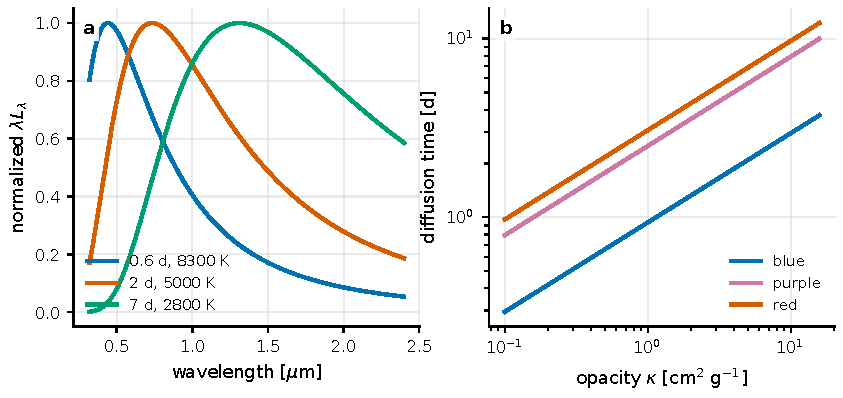
\includegraphics[width=0.92\linewidth]{figures/generated/chapter_13/ch13_kilonova_color_evolution.pdf}
\caption{千新星从蓝到红的演化。左图用三个黑体 SED 标示温度降低后峰值波长向红外移动；右图用扩散时间公式显示 opacity 越大、质量越大、速度越低，峰值越晚。GW170817 的蓝组分快而低 opacity，红组分慢而高 opacity，因此单一 ejecta 组分无法同时解释早期蓝光和晚期 NIR。}
\label{fig:chapter-13-kilonova}
\end{figure}

引力波还给出标准警报器距离。低红移下可粗略写成
\begin{equation}
  H_0\simeq \frac{cz_{\rm host}}{D_L},
  \label{eq:ch13-standard-siren}
\end{equation}
\begin{formulaexplain}
\(H_0\) 是 Hubble 常数，\(z_{\rm host}\) 是宿主红移，\(D_L\) 是引力波给出的光度距离。标准警报器用距离和红移直接测宇宙膨胀率。
\end{formulaexplain}
\(z_{\rm host}\) 是宿主星系红移，\(D_L\) 是从引力波振幅推断的 luminosity distance。GW170817 的主要退化来自 inclination 和 distance：面对面的 binary 既更亮也更难确定倾角。电磁 counterpart 提供宿主、红移、喷流视角和 ejecta 几何，从而减少一部分退化。多信使分析把同一物理事件的这些投影放进一个联合似然。

\section{GRB 余辉怎样把喷流几何写进光变}

GRB prompt emission 给出高能触发，afterglow 给出外激波的可追踪物理。一个相对论 shell 撞入外部介质后，观测时刻 \(t\) 与半径 \(R\) 和 Lorentz factor \(\Gamma\) 的关系近似为
\begin{equation}
  t\simeq \frac{(1+z)R}{4\Gamma^2c}.
  \label{eq:ch13-grb-arrival-time}
\end{equation}
\begin{formulaexplain}
\(t\) 是观测到达时刻，\(R\) 是激波半径，\(\Gamma\) 是 Lorentz 因子。相对论 beaming 让大半径外激波被压缩到很短观测时间。
\end{formulaexplain}
同样的半径，因为 relativistic beaming 和 light-travel-time effect，会被压缩到更短的观测时间。典型 early afterglow 有 \(\Gamma\sim10-300\)，\(R\sim10^{16}-10^{18}\,\mathrm{cm}\)，光学可在触发后几十秒到几分钟进入望远镜视场 \citep{1997ApJ...476..232M,1998ApJ...497L..17S,1998Natur.395..670G,1999PhR...314..575P,2004RvMP...76.1143P,2006ARA&A..44..507W}。

若电子能谱为
\begin{equation}
  N(\gamma_e)\,d\gamma_e \propto \gamma_e^{-p}\,d\gamma_e,
  \qquad \gamma_e>\gamma_m,
  \label{eq:ch13-electron-powerlaw}
\end{equation}
\begin{formulaexplain}
\(N(\gamma_e)\) 是电子 Lorentz 因子分布，\(p\) 是能谱指数，\(\gamma_m\) 是低能截止。同步余辉谱斜率主要由 \(p\) 控制。
\end{formulaexplain}
同步辐射谱在 \(\nu_m\) 和 \(\nu_c\) 附近出现 break。常用观测形式为
\begin{equation}
  F_\nu(t)\propto t^{-\alpha}\nu^{-\beta}.
  \label{eq:ch13-afterglow-powerlaw}
\end{equation}
\begin{formulaexplain}
\(F_\nu(t)\) 是余辉通量密度，\(\alpha\) 是时间衰减指数，\(\beta\) 是谱指数。观测通常先把光变和颜色压缩成这两个斜率。
\end{formulaexplain}
在均匀介质、adiabatic、slow-cooling 且 \(\nu_m<\nu<\nu_c\) 的区间，
\begin{equation}
  \beta=\frac{p-1}{2},
  \qquad
  \alpha=\frac{3(p-1)}{4}.
  \label{eq:ch13-closure-relation}
\end{equation}
\begin{formulaexplain}
closure relation 把观测斜率 \(\alpha,\beta\) 和电子指数 \(p\) 联系起来。若数据偏离它，说明介质、冷却区间或能量注入假设可能不成立。
\end{formulaexplain}
若 \(p=2.2\)，则 \(\beta\simeq0.6\)、\(\alpha\simeq0.9\)。在 \(\nu>\nu_c\) 时常变为 \(\alpha=(3p-2)/4\)。这些 closure relations 的假设很明确：外部介质简单、能量注入不强、microphysical parameters 不剧烈演化、观测频段没有跨过 break。观测上，光学 afterglow 在爆发后一天常为 \(19-20\) mag；偏振可达百分之几到约 \(10\%\)，与同步辐射和喷流几何有关 \citep{2004RvMP...76.1143P,2006ARA&A..44..507W}。

\begin{figure}[tbp]
\centering
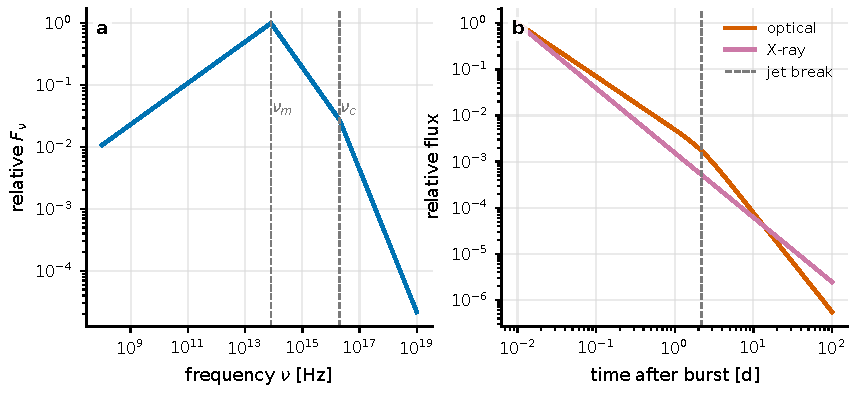
\includegraphics[width=0.92\linewidth]{figures/generated/chapter_13/ch13_afterglow_synchrotron_breaks.pdf}
\caption{GRB afterglow 的同步辐射读法。左图显示 \(\nu_m\) 和 \(\nu_c\) 把谱分成不同斜率区间；右图显示喷流 break 前后光变曲线变陡。若光学和 X-ray 不在同一谱段，它们的 \(\alpha\) 和 \(\beta\) 不必相同，需要先判断观测频率相对 \(\nu_m\)、\(\nu_c\) 的位置。}
\label{fig:chapter-13-afterglow}
\end{figure}

当 \(\Gamma\) 降到约 \(1/\theta_j\) 时，观测者开始看到喷流边缘，光变曲线出现 achromatic jet break。常用估算为
\begin{equation}
  \theta_j\simeq
  0.10
  \left(\frac{t_j}{1\,{\rm d}}\right)^{3/8}
  \left(\frac{1+z}{2}\right)^{-3/8}
  \left(\frac{E_{\rm iso,52}}{n_0}\right)^{-1/8},
  \label{eq:ch13-jet-opening-angle}
\end{equation}
\begin{formulaexplain}
\(\theta_j\) 是喷流半张角，\(t_j\) 是 jet break 时间，\(E_{\rm iso}\) 和 \(n_0\) 是各向同性能量和外部密度。break 越晚，喷流通常越宽。
\end{formulaexplain}
\(\theta_j\) 以 rad 为单位，\(t_j\) 是 break time，\(E_{\rm iso,52}=E_{\rm iso}/10^{52}\,\mathrm{erg}\)，\(n_0\) 是外部介质数密度的 \(\mathrm{cm^{-3}}\) 数值。系数随模型细节而变，但弱指数控制了误差传播：即使 \(E_{\rm iso}\) 或 \(n\) 不确定一个数量级，\(\theta_j\) 也只变几十个百分点。主要风险来自误分类：chromatic break、能量注入、密度跳变或 supernova bump 都可能被误判为 jet break \citep{2003Natur.423..847H,2004ApJ...611.1005G}。

GRB 980425/SN 1998bw 和 GRB 030329/SN 2003dh 把长 GRB 与 broad-lined Type Ic 超新星联系起来；短 GRB 与 BNS merger 的联系在 GW170817 后变成了直接多信使事实。GRB 要求望远镜系统处理极端时间层级：秒级高能触发、分钟级光学 flash、小时到天的 afterglow、周到月的 radio calorimetry，以及可能叠加的 supernova 或 kilonova。事件表除了 flux，还要保留每个阶段的时间基准和频段连接。

\section{TDE 怎样从回落率和再处理光球读出黑洞质量}

潮汐瓦解事件发生在恒星靠近超大质量黑洞时。潮汐半径为
\begin{equation}
  r_t\simeq R_\ast\left(\frac{M_\bullet}{M_\ast}\right)^{1/3},
  \label{eq:ch13-tidal-radius}
\end{equation}
\begin{formulaexplain}
\(r_t\) 是潮汐半径，\(M_\bullet\) 是黑洞质量，\(M_\ast,R_\ast\) 是恒星质量和半径。恒星进入这个半径内会被黑洞潮汐力撕裂。
\end{formulaexplain}
\(M_\bullet\) 是黑洞质量，\(M_\ast\) 和 \(R_\ast\) 是恒星质量和半径。Schwarzschild 半径为
\begin{equation}
  r_s=\frac{2GM_\bullet}{c^2}.
  \label{eq:ch13-schwarzschild-radius-tde}
\end{equation}
\begin{formulaexplain}
\(r_s\) 是 Schwarzschild 半径。比较 \(r_t\) 和 \(r_s\) 可判断恒星是先被潮汐撕裂，还是在亮 flare 前直接落入黑洞。
\end{formulaexplain}
当 \(r_t\lesssim r_s\) 时，恒星可在产生明亮 flare 前被吞没；主序星 TDE 因而最常见于 \(M_\bullet\sim10^5-10^7M_\odot\)，到 \(10^8M_\odot\) 附近选择效应变强 \citep{1988Natur.333..523R,2021ARA&A..59...21G}。

最早返回的 bound debris 给出 fallback time：
\begin{equation}
  t_{\rm min}\simeq
  41\,{\rm d}
  \left(\frac{M_\bullet}{10^6M_\odot}\right)^{1/2}
  \left(\frac{M_\ast}{M_\odot}\right)^{-1}
  \left(\frac{R_\ast}{R_\odot}\right)^{3/2}.
  \label{eq:ch13-tde-fallback-time}
\end{equation}
\begin{formulaexplain}
\(t_{\rm min}\) 是最早 bound debris 返回近心点的时间。它随黑洞质量约按 \(M_\bullet^{1/2}\) 增长，是 TDE rise time 的重要标尺。
\end{formulaexplain}
理想情况下，晚期回落率为
\begin{equation}
  \dot M_{\rm fb}\simeq
  \frac{M_\ast}{3t_{\rm min}}
  \left(\frac{t}{t_{\rm min}}\right)^{-5/3}.
  \label{eq:ch13-tde-fallback-rate}
\end{equation}
\begin{formulaexplain}
\(\dot M_{\rm fb}\) 是 debris 回落率。理想 \(t^{-5/3}\) 衰减是 TDE 的经典标志，但观测光度还会受 circularization 和再处理影响。
\end{formulaexplain}
\(\dot M_{\rm fb}\) 的单位常用 \(M_\odot\,\mathrm{yr^{-1}}\)。Eddington accretion rate 为
\begin{equation}
  \dot M_{\rm Edd}
  =
  \frac{L_{\rm Edd}}{\eta c^2}
  \simeq
  0.022
  \left(\frac{M_\bullet}{10^6M_\odot}\right)
  \left(\frac{\eta}{0.1}\right)^{-1}
  M_\odot\,{\rm yr^{-1}} ,
  \label{eq:ch13-eddington-rate}
\end{equation}
\begin{formulaexplain}
\(\dot M_{\rm Edd}\) 是 Eddington 吸积率，\(\eta\) 是辐射效率。把 \(\dot M_{\rm fb}\) 和它比较，可判断回落是否进入超 Eddington 阶段。
\end{formulaexplain}
\(\eta\) 是辐射效率。对 \(10^6M_\odot\) 黑洞，太阳型恒星的 peak fallback 可以显著超 Eddington，但光学光度未必同样超 Eddington，因为 circularization、wind、obscuration 和 reprocessing 会把内盘能量重分配到 UV/optical。

\begin{figure}[tbp]
\centering
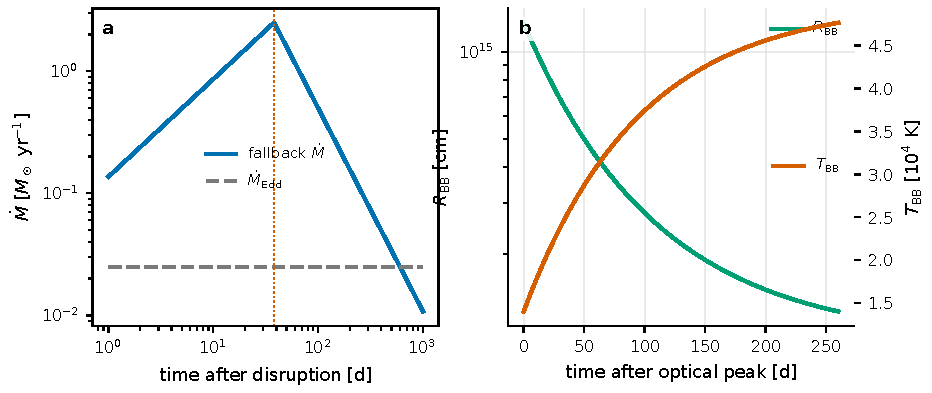
\includegraphics[width=0.92\linewidth]{figures/generated/chapter_13/ch13_tde_fallback_reprocessing.pdf}
\caption{TDE 的回落和再处理。左图显示 \(t^{-5/3}\) fallback 在几十天尺度进入衰减段，并可长期高于 \(10^6M_\odot\) 黑洞的 Eddington accretion rate。右图给出 optical/UV 黑体光球的一种典型演化：半径从 \(10^{15}\,\mathrm{cm}\) 量级收缩到 \(10^{14}\,\mathrm{cm}\)，温度从 \(10^4\,\mathrm{K}\) 量级升到数 \(10^4\,\mathrm{K}\)。}
\label{fig:chapter-13-tde}
\end{figure}

光学 TDE 的黑体半径通常为 \(10^{14}-10^{15}\,\mathrm{cm}\)，比 \(10^6M_\odot\) 黑洞的几倍 \(r_s\) 大得多；温度常为几 \(10^4\,\mathrm{K}\)，演化比普通超新星慢。AT2018zr 是 ZTF 早期样本中第一个有很好 rise-to-peak 覆盖的 TDE，最早 ZTF 检测约在峰值前 \(50\,\mathrm{d}\)。其光学/UV 黑体温度早期约 \(1.4\times10^4\,\mathrm{K}\)，晚期可升到 \(>5\times10^4\,\mathrm{K}\)，黑体半径从 \(10^{15.1}\,\mathrm{cm}\) 降到 \(<10^{14}\,\mathrm{cm}\)；X-ray luminosity 比同时期 optical/UV blackbody luminosity 低数个数量级，说明 obscuration 或 reprocessing 不能忽略 \citep{2019ApJ...872..198V,2021ARA&A..59...21G}。

喷流型 TDE 例如 Swift J1644+57 则把事件表推向高能和快速变率：X-ray 可强烈闪烁，radio emission 跟踪 outflow 与外部介质相互作用 \citep{2011Sci...333..203B}。IceCube-170922A 和 blazar 的多信使联系属于另一类源；TDE 中也有高能 neutrino 关联的候选个例 \citep{2021NatAs...5..510S}。在长时标瞬变里，事件表仍然要保留完整时间信息。判断一个高能事件是否属于 optical flare，需要同时看天球位置、时间延迟、能量、方向误差和源演化是否相容。

\section{机会目标观测怎样避免只抢快不算误差}

瞬变观测成败常由响应时间决定。一个实用条件是
\begin{equation}
  t_{\rm alert}+t_{\rm slew}+t_{\rm acq}+t_{\rm exp}
  < f_{\rm samp}\,t_{\rm evol},
  \label{eq:ch13-response-budget}
\end{equation}
\begin{formulaexplain}
左边是从触发到第一组有效曝光的总响应时间，右边是希望采样的源变化时间。机会目标观测要把“快”量化成这个预算。
\end{formulaexplain}
\(t_{\rm alert}\) 是触发发布延迟，\(t_{\rm slew}\) 是望远镜转向，\(t_{\rm acq}\) 是目标确认和导星，\(t_{\rm exp}\) 是第一组有效曝光，\(t_{\rm evol}\) 是源变化时标。若希望解析上升段，\(f_{\rm samp}\sim0.1\) 比较合理。GRB optical flash 的 \(t_{\rm evol}\) 可小于 \(10^3\,\mathrm{s}\)，GW counterpart 的蓝光阶段约一天，新星早期射电/光谱结构可在天到周内变化，TDE 的 rise time 则常为数十天。

普通成像曝光的信噪比为
\begin{equation}
  {\rm SNR}=
  \frac{N_s}
  {\left(N_s+N_b+n_{\rm pix}\sigma_{\rm read}^2\right)^{1/2}},
  \label{eq:ch13-imaging-snr}
\end{equation}
\begin{formulaexplain}
\({\rm SNR}\) 是成像信噪比，\(N_s\) 是源计数，\(N_b\) 是背景计数，读出噪声按像素数累加。曝光选择要同时看源、背景和读出噪声。
\end{formulaexplain}
\(N_s\) 是源计数，\(N_b\) 是背景计数，\(n_{\rm pix}\) 是 aperture 内像素数，\(\sigma_{\rm read}\) 是每像素读出噪声。强度干涉或 photon-pair 统计还要看 pair 数：
\begin{equation}
  N_{\rm pair}\simeq r_1 r_2\,\Delta t\,T,
  \qquad
  \delta C\simeq N_{\rm pair}^{-1/2},
  \label{eq:ch13-pair-statistics}
\end{equation}
\begin{formulaexplain}
\(N_{\rm pair}\) 是相关窗口内的光子对数，\(r_1,r_2\) 是事件率，\(\Delta t\) 是相关窗口，\(T\) 是累计时间。相关误差按光子对数平方根下降。
\end{formulaexplain}
\(r_1\) 和 \(r_2\) 是两台望远镜的事件率，\(\Delta t\) 是相关窗口，\(T\) 是累计时间。若 \(r_1=r_2=10^6\,\mathrm{s^{-1}}\)、\(\Delta t=100\,\mathrm{ps}\)、\(T=1\,\mathrm{h}\)，则 \(N_{\rm pair}\sim3.6\times10^5\)，纯 Poisson 相关误差约 \(1.7\times10^{-3}\)。这只是统计下限，真实误差还包括时间同步、dead time、光谱带宽、偏振泄漏和背景变化。

宿主关联也有明确的数量级。若瞬变位置误差半径为 \(r\)，深度 \(m\) 内背景星系面密度为 \(\Sigma(<m)\)，随机重合概率可写成
\begin{equation}
  P_{\rm cc}=1-\exp[-\pi r^2\Sigma(<m)].
  \label{eq:ch13-chance-coincidence}
\end{equation}
\begin{formulaexplain}
\(P_{\rm cc}\) 是随机宿主重合概率，\(r\) 是定位误差半径，\(\Sigma(<m)\) 是背景星系面密度。定位越差、星系越密，宿主关联越不可靠。
\end{formulaexplain}
GW170817 的 Virgo 加入把天空定位显著收缩到几十平方度量级，使光学巡天能够在同一夜定位宿主；TDE 选择则需要亚角秒 astrometry 来证明 flare 与星系核一致。AT2018zr 的 ZTF 分析显示，对核瞬变，多个差分检测可把 host-flare offset 的统计误差压到远小于单次 seeing 的尺度 \citep{2017PhRvL.119p1101A,2017ApJ...848L..12A,2019ApJ...872..198V}。

\begin{longtable}{@{}p{0.14\linewidth}p{0.19\linewidth}p{0.27\linewidth}p{0.28\linewidth}@{}}
\toprule
源类 & 关键时标 & 典型观测量 & 主要风险 \\
\midrule
经典新星 & 天到月 & 谱线速度、射电角尺度、\(\gamma\) 射线窗口 & 多速度组分会偏置膨胀视差。 \\
Type Ia & 天到周 & 光变宽度、颜色、Si II 速度、偏振、微角秒角尺度 & 光度校正和角尺度来自不同物理层。 \\
核心坍缩 & 分钟到天 & UV/软 X-ray 暴发、早期光谱、偏振 & 触发太晚会错过前身星半径信息。 \\
千新星 & 小时到十天 & GW 距离、\(\gamma\) 射线延迟、颜色和 NIR 演化 & opacity、视角和 ejecta 几何退化。 \\
GRB & 秒到月 & \(\alpha\)、\(\beta\)、jet break、偏振、radio calorimetry & 色变 break 或能量注入会误判喷流几何。 \\
TDE & 周到年 & rise time、核位置、\(T_{\rm BB}\)、\(R_{\rm BB}\)、X-ray/optical ratio & AGN 变量污染和再处理几何不唯一。 \\
\bottomrule
\end{longtable}

